\section{Modelo de Especificação de Ativos Reutilizáveis}

\subsection{Considerações Iniciais}

    No âmbito da Engenharia de software, a utilização de ativos de softwares reutilizáveis são de grande interesse, visto que a pratica de sua utilização, fornece vantagens e beneficios muito importantes ao desenvolvimento de softwares, como melhoria de qualidade, aumento de produtividade e redução de custos.
	A biblioteca desenvolvida neste trabalho, possui relação com o modelo de especificação de ativos reutilizáveis (RAS OMG-2005), pois contempla o desenvolvimento de repositórios de ativos de software que estejam de acordo com as orientações do padrão citado. Essa seção explora os principais conceitos que abragem as orientações especificadas no modelo RAS.

\subsection{Definições e Especificações de Ativos de Software}

Um ativo de software segundo a definição da OMG (Object Management Group - 2005), é algo que visa a solução de algum problema em um determinado contexto, possui pontos de variabilidades e regras de como seu reuso pode ser realizado. A figura a seguir ilustra a composição de um ativo de software.

\begin{figure}[H]
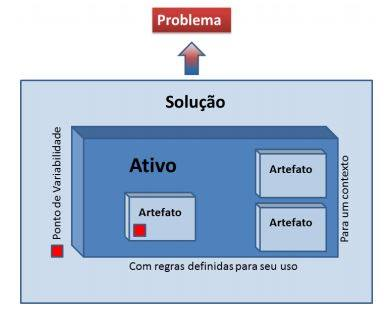
\includegraphics[width=0.5\textwidth]{images/ativo}
\centering
\caption{Ilustração de um ativo de software}
\label{Rotulo}
\end{figure}

  Ou seja, um ativo de software reutilizável é o conjunto que compõe a solução de um determinado problema, sendo composto por diferentes artefatos, que podem ser tanto códigos fontes, quanto documentação de projeto, ferramentas adotadas, entre outros artefatos.
 

    A OMG  utiliza três pontos-chave para descrever os ativos reutilizáveis, que apresentam-se como: Granularidade, Variabilidade e Articulação. A seguir descrevemos a definição de cada um destes.
    
 \begin{itemize}
    \item Granularidade: descreve a quantidade de problemas específicos ou soluções alternativas um pacote de artefatos pode resolver. Ativos mais simples, podem compreender um único problema bem definido. Porém com o aumento da complexidade do ativo em conjunto com o aumento de seu tamanho, a sua capacidade de resoluções de problemas aumenta junto a sua granularidade.
    \item Variabilidade: condiz com a capacidade do ativo fornecer variabilidade. Ou seja a possibilidade de alteração de suas caracteristicas, a OMG exibe as caracteristicas de variabilidade de um ativo por meio de um conjunto formado por quatro tipos:
    \begin{itemize}
         \item \textbf{Ativos caixa-preta:} a sua implementação interna não é conhecida e não pode ser alterada, por exemplo, componentes binários.
        \item \textbf{Ativos caixa-branca:} a sua implementação interna é conhecida e podem ser alterada, por exemplo, códigos fonte.
        \item \textbf{Ativos caixa-clara:} a sua implementação é conhecida, mas não podem ser modificados, por exemplo, documentação, modelos, fragmentos de código.
        \item \textbf{Ativos caixa-cinza:} a sua implementação é conhecida, porém apenas determinados subconjuntos de artefatos podem ser modificados, por exemplo, serviços disponibilizados, que em geral, permitem manipulação por meio de parâmetros.
    \end{itemize}
    
    \item Articulação: condiz com a capacidade do ativo de prover a solução do problema. Um ativo mais completo, constituído por exemplo de documentação, código fonte e testes que fornecem uma solução, possui um alto nível de articulação. 

\end{itemize}

    A biblioteca \textit{Hidra} aborda especificamente a segunda forma de armazenamento de ativos reutilizáveis de software.

\subsection{Ativos de Sotware}

    O RAS é descrito em duas principais categorias, o núcleo RAS e seus Perfis. O núcleo representa os elementos fundamentais para a especificação de uma ativo, e os perfis descrevem extensões desses elementos fundamentais. O perfil de uma ativo não altera a definição semântica de um elemento descrito no núcleo. O núcleo RAS não é instaciavel, assim como uma classe abstrata, portanto um ativo deve possui um perfil particular, esse perfil pode estender o núcleo RAS, ou estender um outro perfil como mostrado na figura a seguir.


\begin{figure}[H]
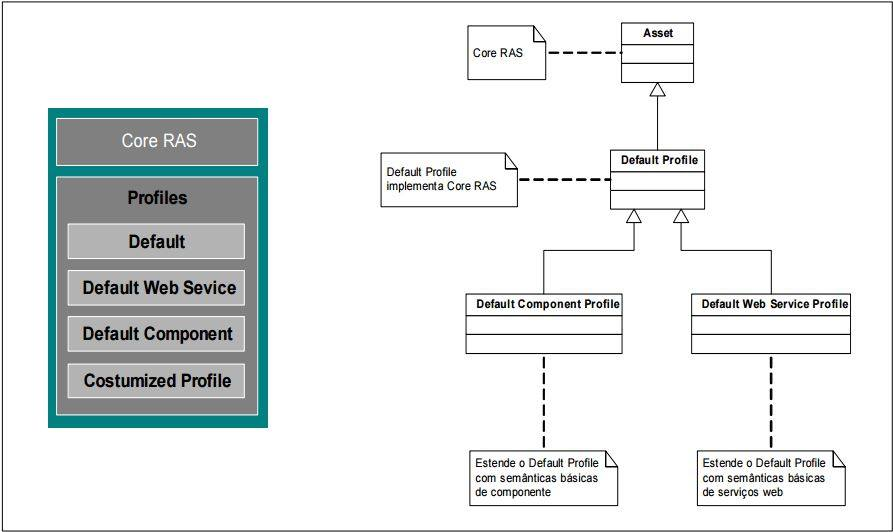
\includegraphics[width=0.8\textwidth]{images/estruturaAsset}
\centering
\caption{Estrutura de um Ativo de Softawe \cite{dissertacaoHenriqueFaria2005}}
\label{Rotulo}
\end{figure}

Um ativo de software é composto pela sua Classificação \textit{(Classification)}, Solução \textit{(Solution)}, Utilização \textit{(Usage)}, e pelo seu Perfil \textit{(Profile)}. Caso esteja relacionado a outros ativos também possuirá (Related Assets). A descrição de cada atributo é informada a seguir:

\begin{itemize}
    \item Classificação \textit{(Classification)}: : um conjunto de descritores que são usados para fazer a classificação do ativo, como descrever os contextos nos quais a reutilização do ativo é relevante.
     \item Solução \textit{(Solution)}: contém as descrições de um ou mais artefatos que fazem parte do ativo.
     \item Utilização \textit{(Soltuion)}: contém as regras para a instalação, customização e uso do ativo, ou seja, possui as instruções correspondentes a cada artefato que o ativo possui e um contexto de referência.
     \item Ativos Relacionados \textit{(Related Assets)}: condiz com as descrições dos relacionamentos existentes entre os ativos.
     \item Perfil \textit{(Profile)}: representa o perfil do ativo.
\end{itemize}
\begin{figure}[H]
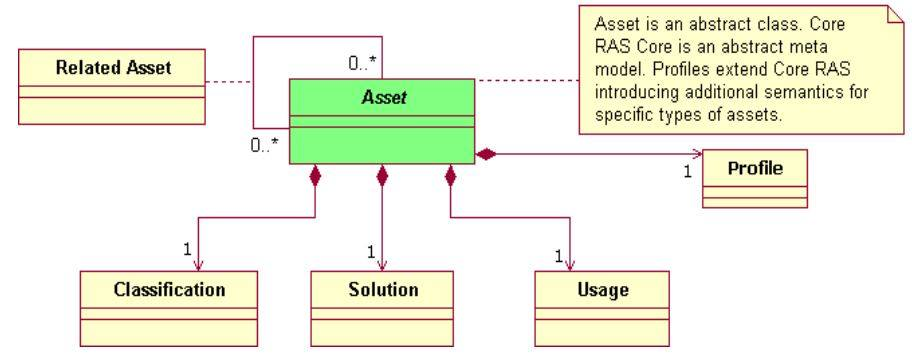
\includegraphics[width=0.8\textwidth]{images/modeloAsset}
\centering
\caption{ Estrutura de um ativo de Software (OMG, 2005)}
\label{Rotulo}
\end{figure}

\subsection{Considerações Finais}
    Nesta seção apresentamos as principais definições e orientações do modelo RAS utilizado como fonte de informação para desenvolvimento deste trabalho. Um dos aspectos abordados pela biblioteca Hidra é a validação, aceitação e persistência, em repositórios de ativos de software, condizentes com o padrão RAS descrito nesta seção.




% \makebox[\width]{Fonte: baseado em \citeonline[p.~4]{fulano}.}}
%     \label{interface}